\documentclass[../vis.tex]{subfiles}

\begin{document}

\subsection{Extension Bundle}
\label{extension}
Technically speaking, \textit{Vizic} is an extension bundle to the Jupyter Notebook App. It comes with a notebook extension and a server extension.
The notebook extension is written in both Python and JavaScript. The Python code mainly consists of the APIs to create interactive widgets and a set of functions to interact with them.
The JavaScript section is the front-end interface that actually constructs the widgets in the browser, and also handles the interactions on the widgets by either sending state changing message to the kernel or responding directly at the front-end.
The Python code that runs in the kernel and its JavaScript counterpart that runs in the browser communicate with each other through the ``comms'' messaging API provided by the Jupyter Notebook.

Beyond the excellent platform offered by Jupyter Notebook, \textit{Vizic} also takes advantage of \textit{ipywidgets} and \textit{ipyleaflet}\footnote{https://github.com/ellisonbg/ipyleaflet}.
\textit{ipywidgets} offers a widget-model-view framework for building widgets within Jupyter notebooks.
All widgets in \textit{Vizic} are built based on the widget-model-view structure.
The widget-model-view structure uses IPython \textit{traitlets}\footnote{https://traitlets.readthedocs.io/en/stable/} to keep attributes or states synchronized at both front and back end and to trigger further actions according to state changes, which makes it possible to complete tasks both interactively using widgets and from the command line within the notebook cells.
IPython \textit{traitlets} is a framework that lets Python classes have attributes with type checking, dynamically calculated default values, and ‘on change’ callbacks. That way the user can build custom widgets to control the state of the sky maps and layers or to run and trigger additional scripts based on state changes. Such flexibility makes \textit{Vizic} even more powerful and extensible.

In addition, \textit{ipyleaflet} is a notebook extension package that integrates the \textit{Leaflet} library into the Jupyter Notebook framework environment.

The server extension is written also in Python using \textit{Tornado}\footnote{http://www.tornadoweb.org/}. This extension connects the kernel and the map widgets to the MongoDB database.
Whenever the front-end sky map asks for new data, the request will go through the server extension and return with the query results.
To enhance the performance, we used \textit{Motor}\footnote{https://motor.readthedocs.io}, an asynchronous Python driver for MongoDB, to access the database from the server.
As a result, multiple tiles on a map can be loaded concurrently, and multiple maps visualizing different catalogs can be displayed in one single notebook without a heavy performance cost.
\subsection{Slippy Map}
\begin{figure}[h]
  \centering
  %\textbf{Selection Tool}\par\medskip
  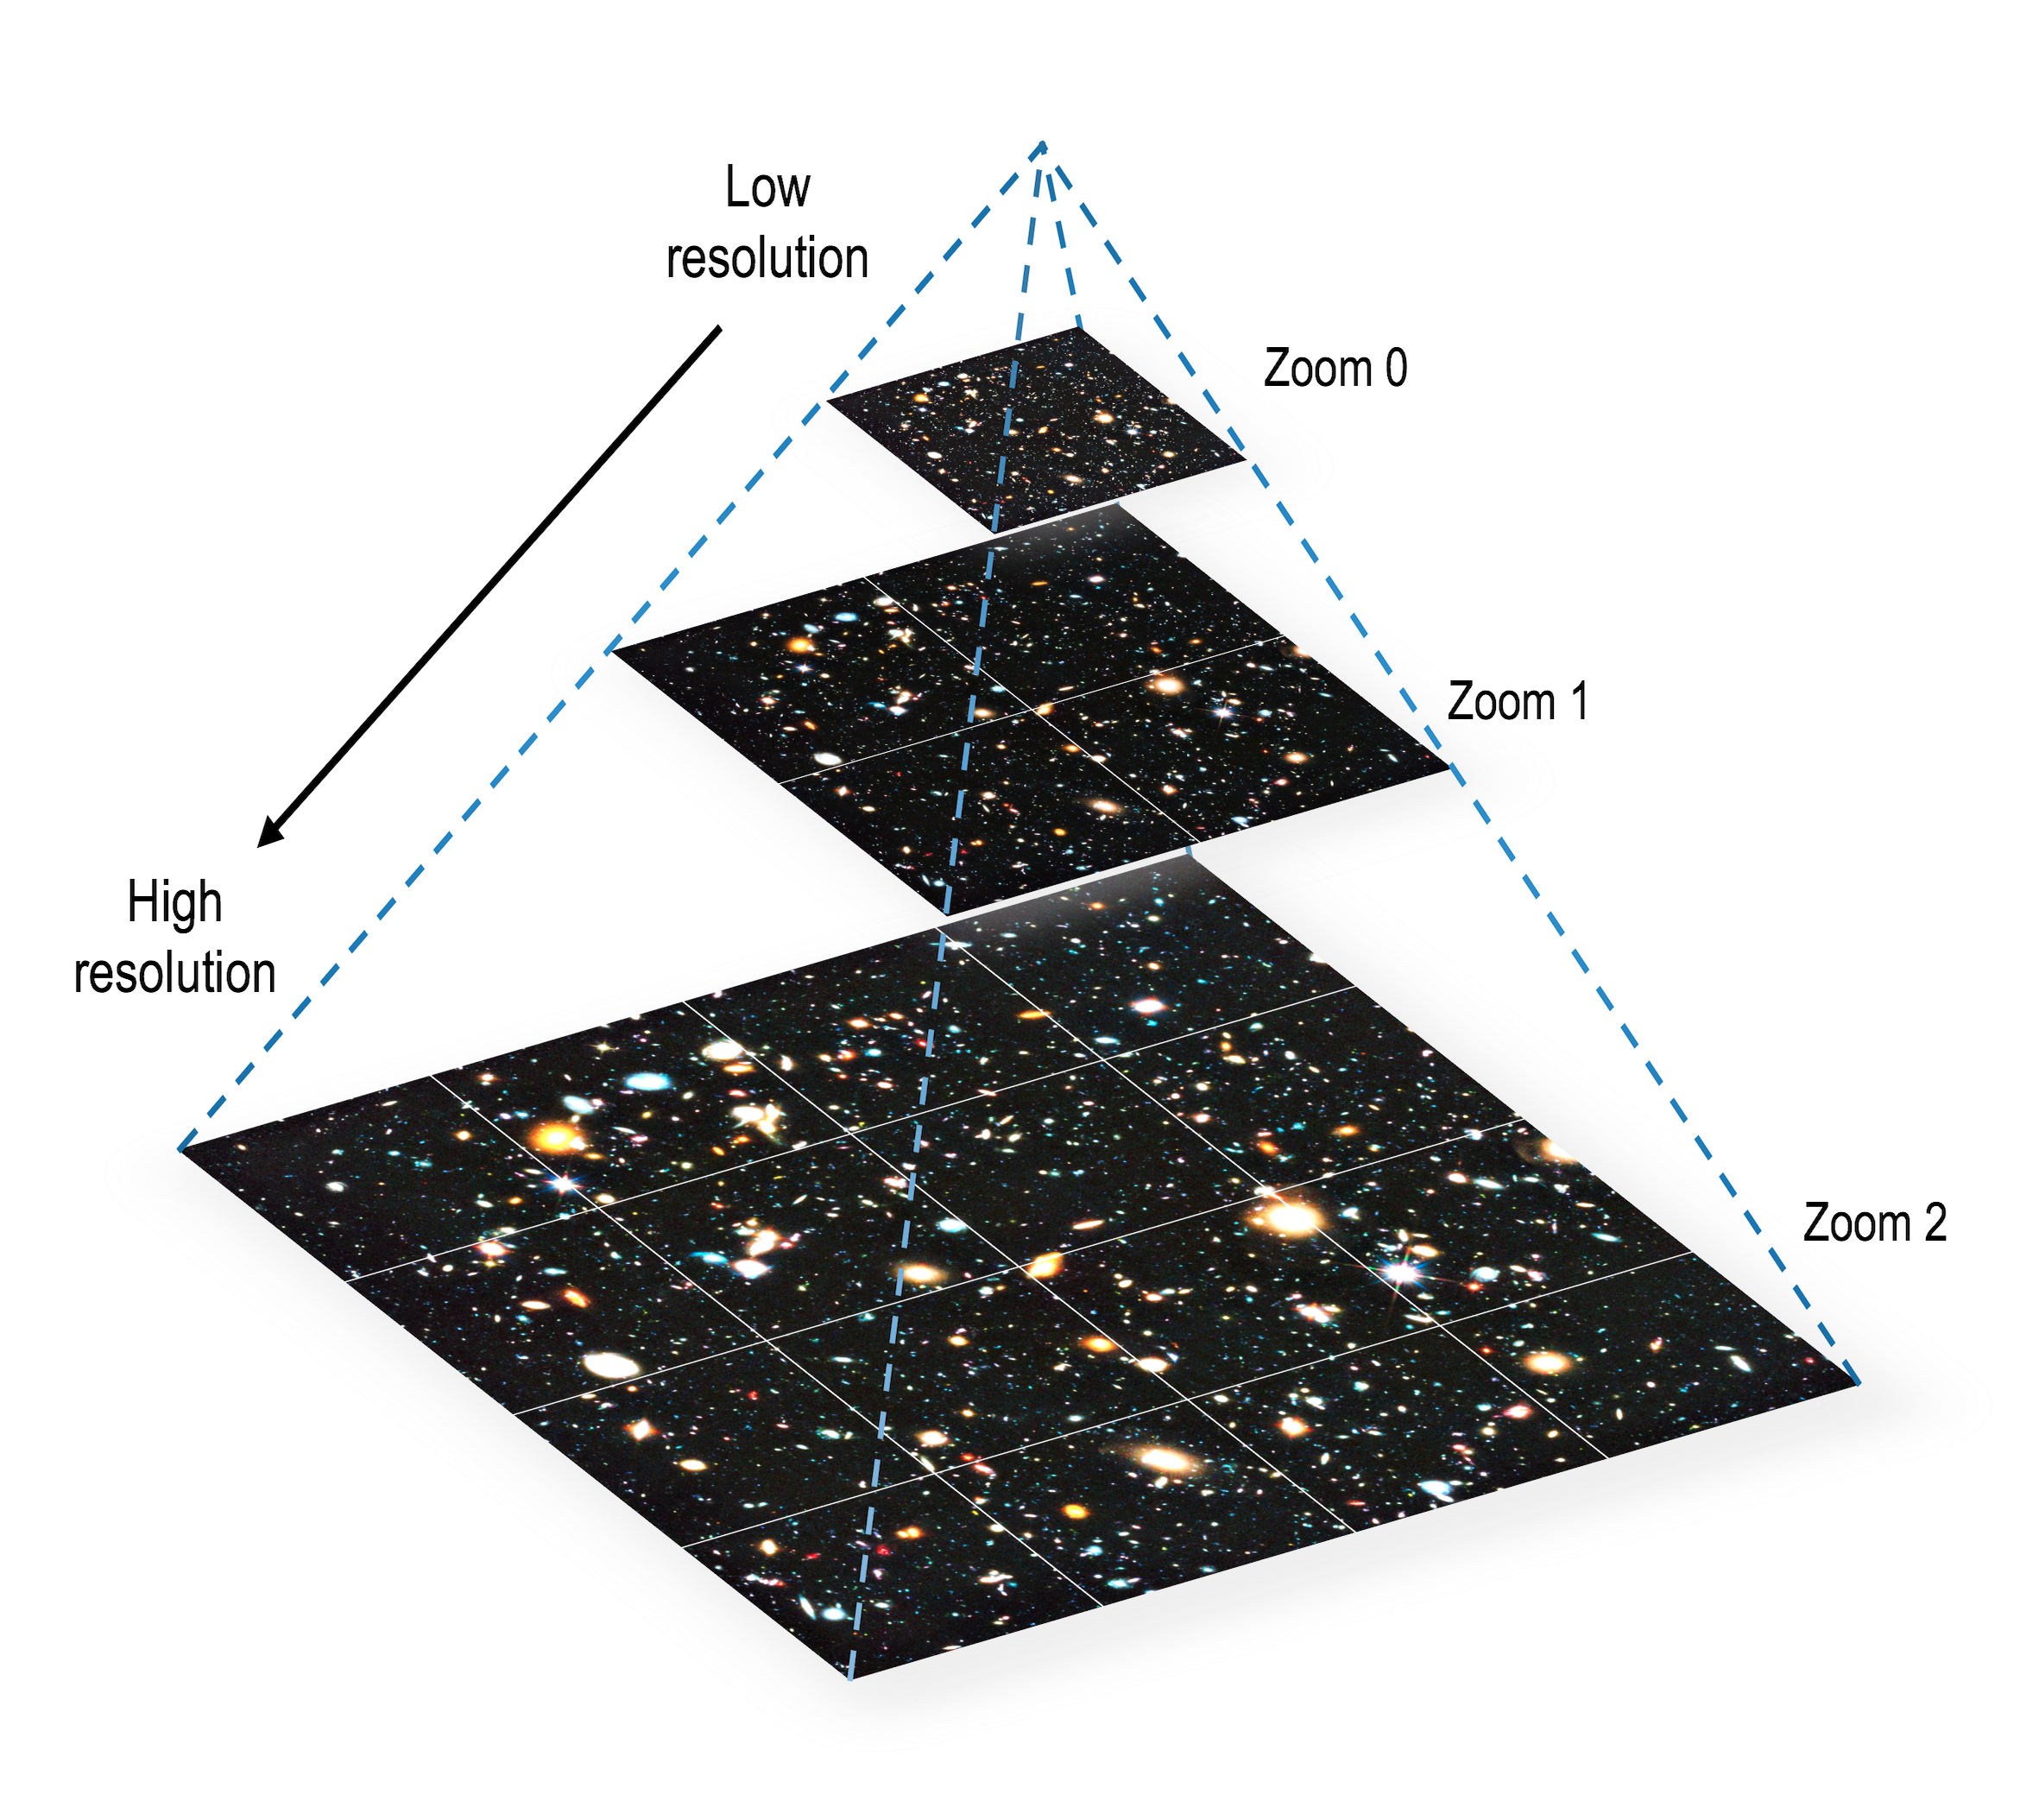
\includegraphics[width=0.45\textwidth]{FIG8}
  \captionsetup{width=0.45\textwidth}
  \caption{3D diagram explaining the pyramid like structure of the tiles system. Image Credit: NASA, ESA, H. Teplitz and M. Rafelski (IPAC/Caltech), A. Koekemoer (STScI), R. Windhorst (Arizona State University), and Z. Levay (STScI)}
  \label{fig:tilepyramid}
\end{figure}
\begin{figure}[h!]
  \centering
  %\textbf{Selection Tool}\par\medskip
  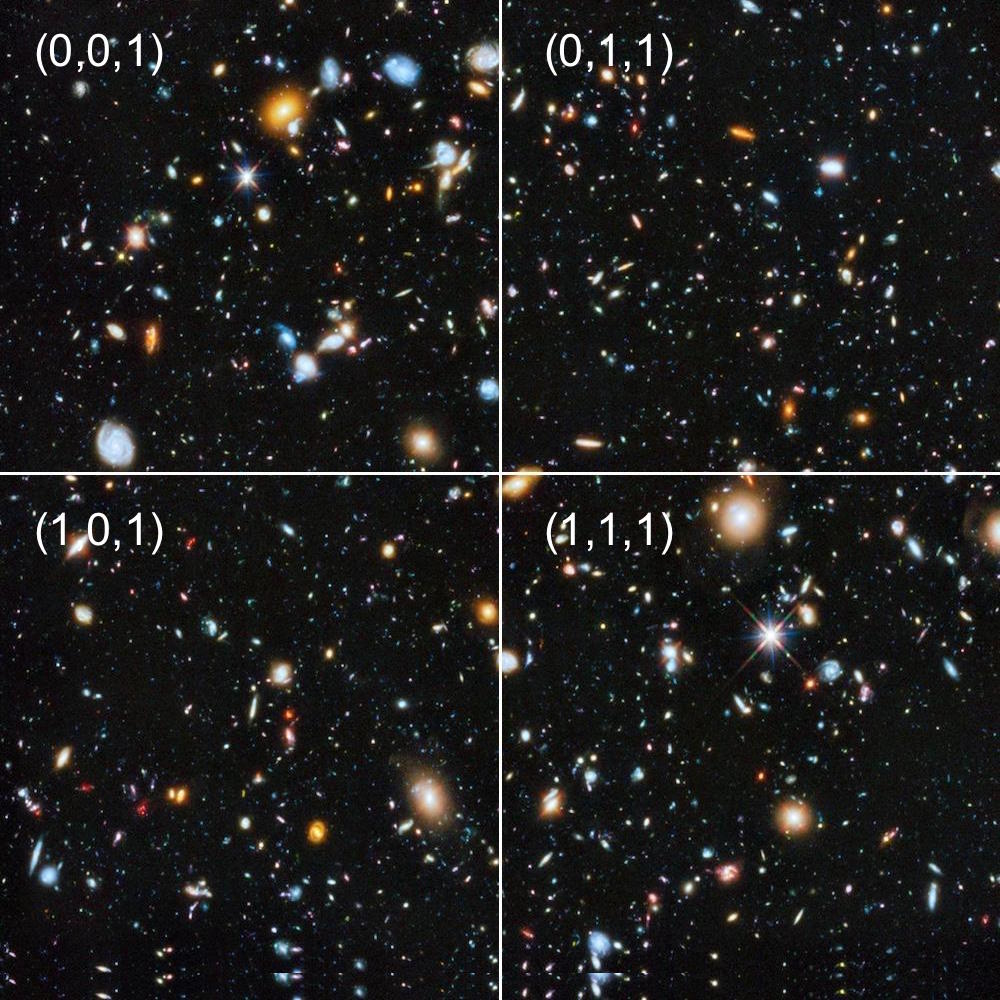
\includegraphics[width=0.4\textwidth]{FIG9}
  \captionsetup{width=0.45\textwidth}
  \caption{A figure showing the coordinate system used to locate the tiles. Image Credit: NASA, ESA, H. Teplitz and M. Rafelski (IPAC/Caltech), A. Koekemoer (STScI), R. Windhorst (Arizona State University), and Z. Levay (STScI)}
  \label{fig:coord}
\end{figure}

The main concept that stands behind the interactive maps created by \textit{Vizic} is the ``slippy map'' implementation.
The ``slippy map'' or tiled web map is the standard method of serving large maps on the web.
A well-known example adopting this approach is Google Maps. For a better illustration of the ``slippy map'' mechanism, we have constructed a 3-D diagram of its pyramid-like data structure using a Hubble image as an example (note that \textit{Vizic} does not display images), and with the diagram shown in Figure \ref{fig:tilepyramid}.
The images at different zoom levels are identical in terms of content but with different resolutions.
The higher the zoom level, the higher the resolution of the image. At each zoom level, the image is divided into many small square tiles, each with a size of $256 \times 256$ pixel.
The number of tiles at zoom level $n$ is be determined by
\begin{equation*}
N_{tile} = 2^{n} \times 2^{n}
\end{equation*}
\label{slippy}

Since the map window on our monitor is fixed, the number of small tiles that the window can display is relatively stable.
The JavaScript engine at the front-end only needs to request the tiles that can be displayed and disregard the rest for efficiency.
The initial idea behind this algorithm is that for an image that is much larger than the size of map window measured pixels, a big portion of this image is hidden at high zoom levels, which makes it very inefficient to load the entire image to the client side.
However, at lower zoom levels, many pixels are compressed into a single pixel on the display, therefore we are not able to perceive the information offered by the full-resolution image.
The ``slippy map'' implementation avoids the heavy loads by offering a pyramid-like multi-resolution structure, which in fact has been proved to be very efficient.
In order to correctly locate and request the tiles for \textit{Vizic}, each tile is also assigned an ID following the pattern $ (x, y, z) $, where $x$ and $y$ are row number and column number respectively and $z$ is the zoom level (see Figure \ref{fig:coord}).


Traditionally, in an interactive map, each tile is a PNG image, we have made a step forward by vectorizing these tiles before display.
We store each object in the catalog as a document in the MongoDB database and create the visual representations on the fly.
Before importing the catalog into the database, we split the data into $2^{n}*2^{n}$ groups following a similar grid as shown in Figure \ref{fig:coord} , where $n$ is the maximum zoom level with a default value of $8$, which can be changed at the catalog ingestion process.
Each group represents a tile at the maximum zoom level and objects in that group is assigned the tile ID of the group.
When a lower zoom level tile is requested, the ID for the requested tile is translated into a set of tile IDs at the maximum zoom level. This way we can further reduce the size and complexity of the data stored in the database.
The projection functions are shown below:
\begin{align*}
x_{max} &= xc*2^{z_{max}-z}-1\\
x_{min} &= (xc+1)*2^{z_{max}-z}\\
y_{max} &= yc*2^{z_{max}-z}-1\\
y_{min} &= (yc+1)*2^{z_{max}-z}
\end{align*}

$ x_{max}, x_{min}, y_{max}, y_{min} $ are the maximum and minimum values of $x$ and $y$ in the tile ID respectively.
$z_{max}$ is the maximum zoom level and $z$ is the zoom level of the requested tile.
At lower zoom levels, we reduce the load by leaving out objects that are too small to see (i.e., not resolved by the screen).

In particular, objects that have a semi-minor axis (or radius) smaller than one third of a pixel after being projected onto the screen will not be included in the data query. Here the number one third of a pixel is chosen because it provides extra tolerance for conversion offsets than one half of a pixel.
A shape that is smaller that one pixel either has a very low opacity or becomes invisible on the screen, so it is unnecessary to spend resource on those objects.
By projecting tile coordinates and leaving out invisible objects, we have successfully emulated the ``slippy map'' implementation in a vectorized way for catalog data.

The ``slippy map'' implementation is ideal for both displaying static images and displaying vectorized data, however the current scope of \textit{Vizic} is not to display static images. Even though, \textit{Vizic} can be extended to display both images and catalogs in the same manner.
\subsection{Custom Overlays}
\label{overlay_mech}
\begin{figure}[h]
  \centering
  %\textbf{Selection Tool}\par\medskip
  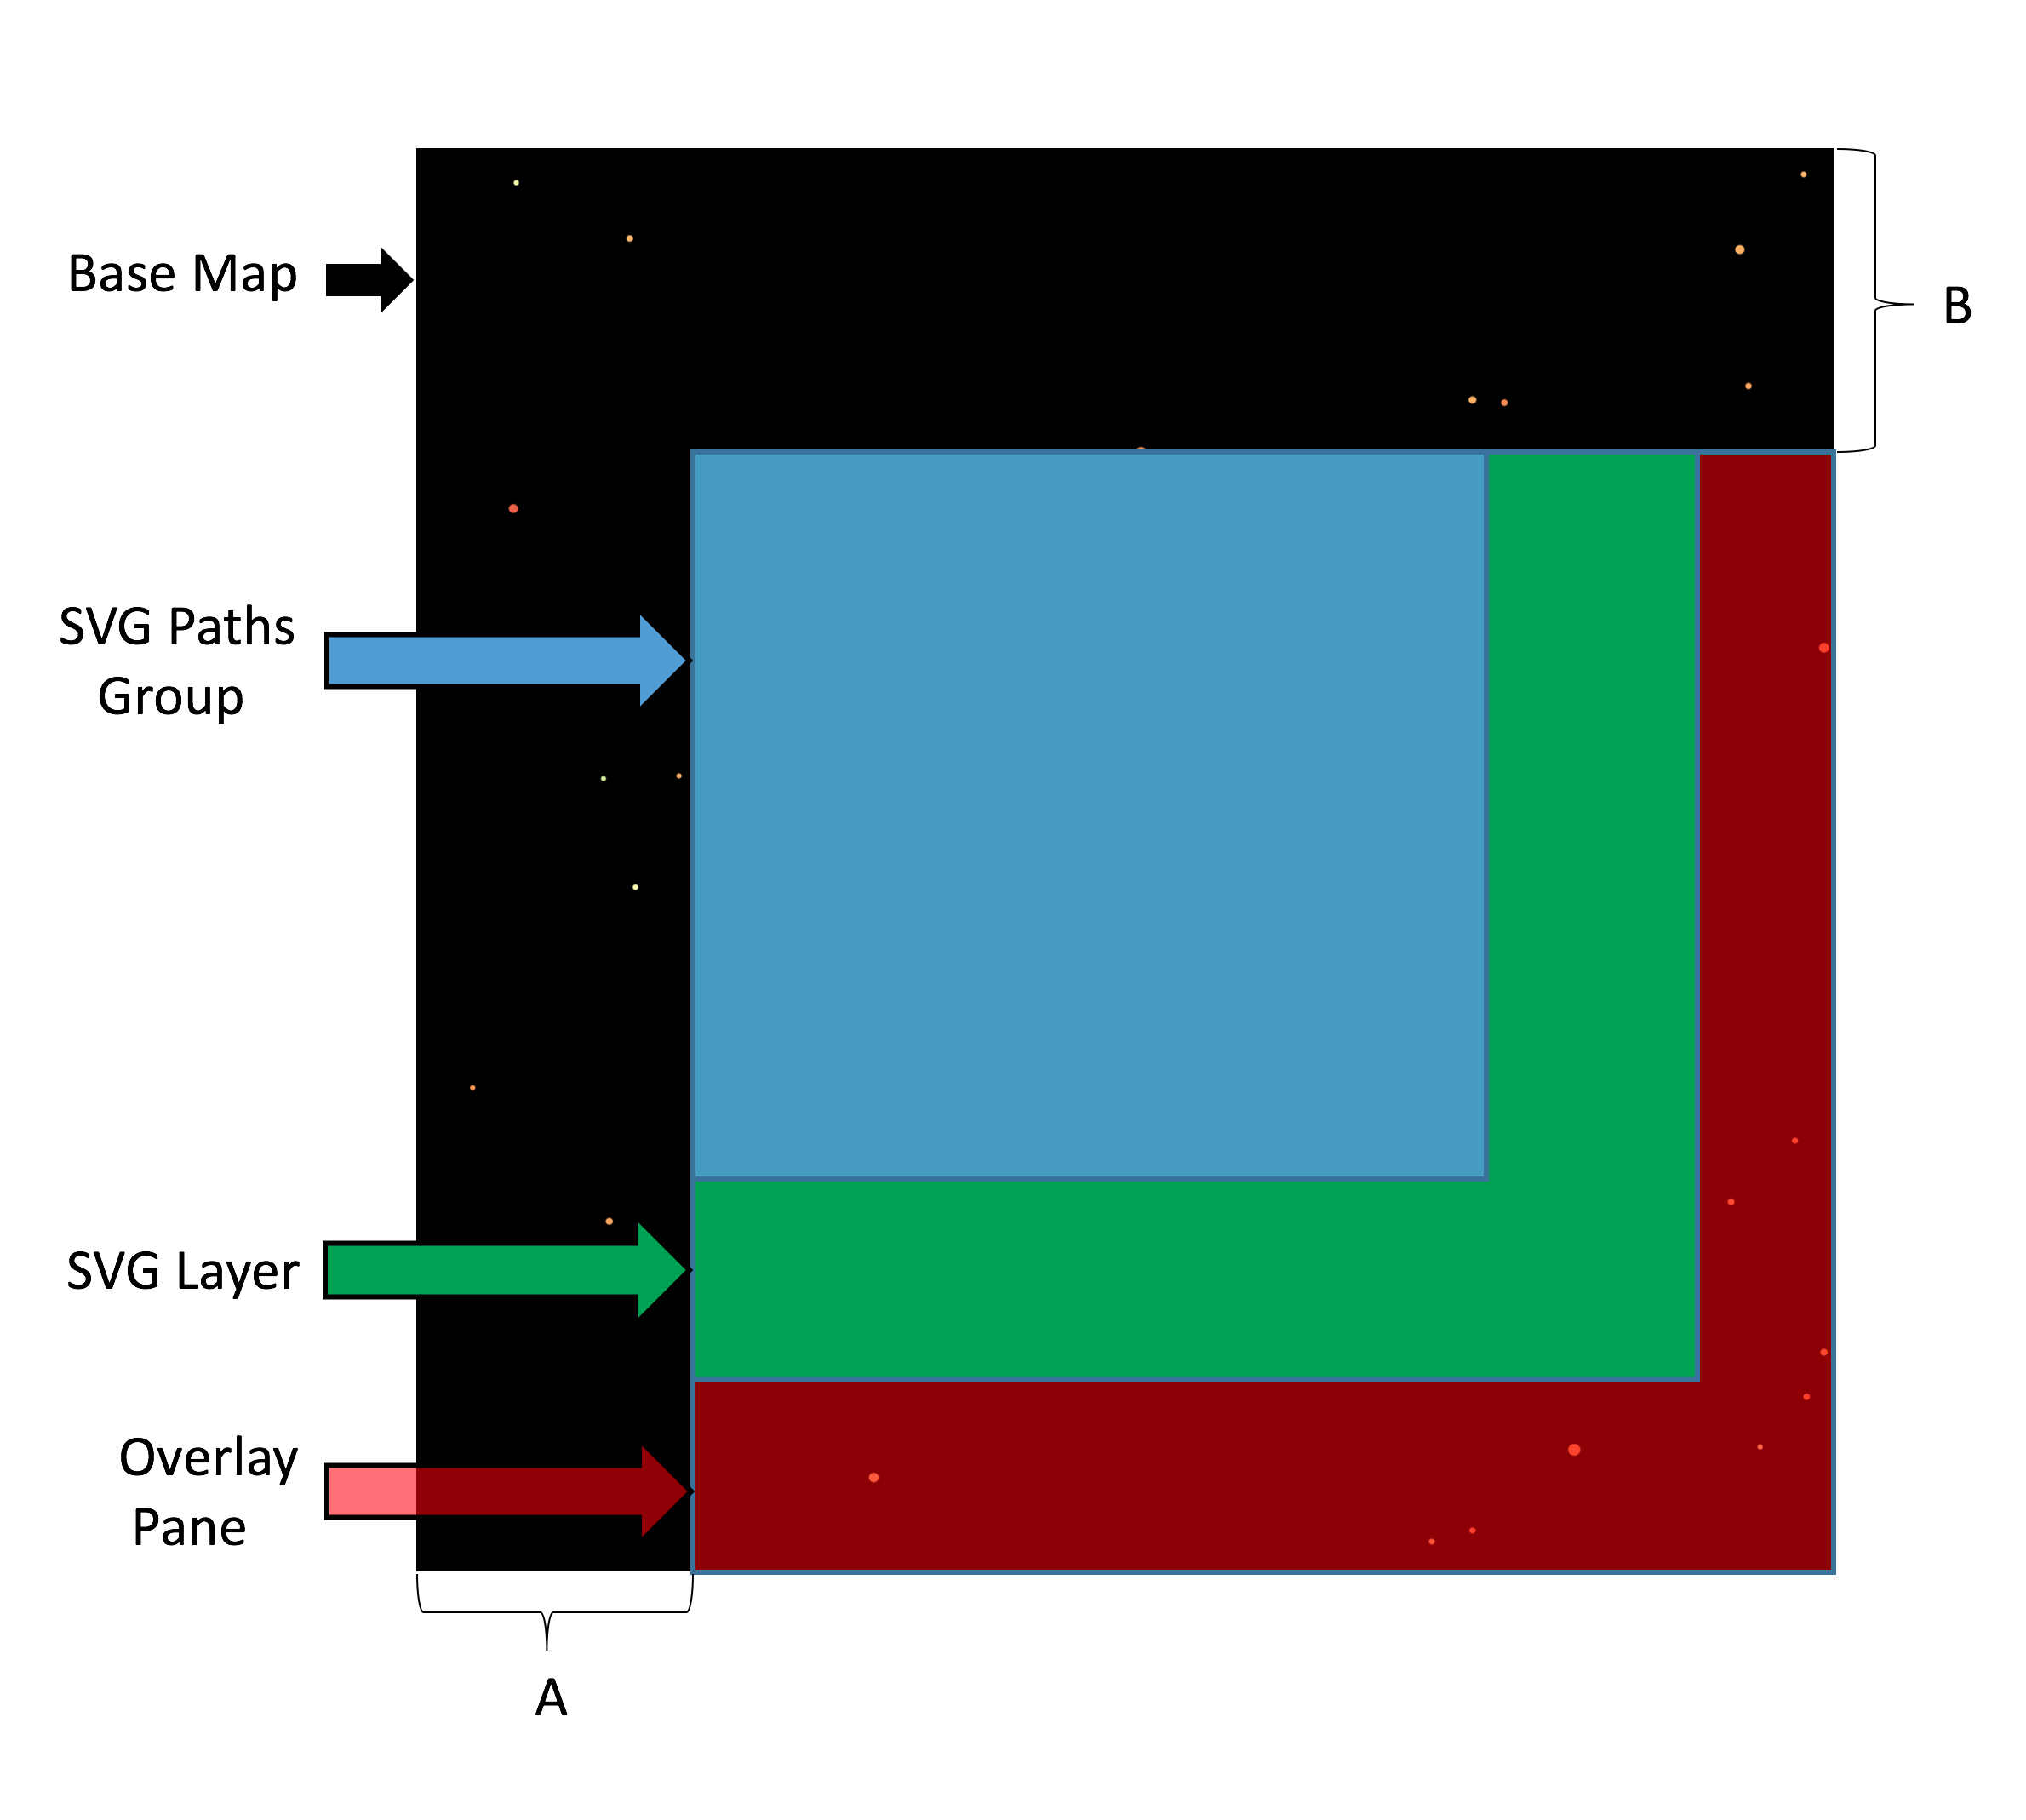
\includegraphics[width=0.45\textwidth]{FIG10}
  \captionsetup{width=0.45\textwidth}
  \caption{A diagram displays the layer structure of the mapping system. A is the offset in longitude direction. B is the offset in latitude direction.}
  \label{fig:layerdiagram}
\end{figure}
As described in Section \ref{adv}, \textit{Vizic} allows custom overlays to be appended on top of the visualized catalogs.
We make this possible by extending the \texttt{Layer} class in \textit{Leaflet} and providing specific drawing constructions based on the type of geometric shape contained in the overlay.
Since it is unpractical to redraw the overlay using canvas element every time the viewport changes (e.g., zoom and pan), we instead create the overlay with a collection of SVG elements.
SVG elements are vector-based, therefore we only need to create them once and resize them as the map size changes.
Because the \textit{Leaflet} map is a multi-layered system (see Figure \ref{fig:layerdiagram}), to accommodate the offsets generated by rescaling of the overlay when zoom level changes, we put these SVG elements into a group element, and scale and shift them together.
The offsets are determined as follows:
\begin{align*}
A &= lon_{base} - lon_{op}\\
B &= lat_{base} - lat_{op}
\end{align*}

$A$ and $B$ are the offsets in the longitude and latitude directions, $(lon_{base},lat_{base})$ is the coordinate for the base map and  $(lon_{op},lat_{op})$ is the coordinate for the overlay pane. In \textit{Leaflet}, panes are used to control the ordering of layers on the map. Overlay pane is the default pane for all the vector overlay layers.

\subsection{MongoDB}
\label{mongodb}
\textit{Vizic} uses MongoDB databases to store and serve the catalogs.
MongoDB is a document-oriented database, which stores rows from a traditional RDBMS database into documents to enable faster query and better scalability.
Considering astronomical catalogs are simply collections of observed objects without complex relations between each columns when it comes to visualizing them, and since \textit{Vizic} only asks for objects and their properties from a catalog using their positions in the sky, MongoDB is a better choice comparing to a traditional RDBMS database.

\textit{Vizic} stores the data for each object in a document, each collection of documents is a catalog and each database can contain many collections.
Every document is indexed by its tile ID and the size of the object measured in arcsecond to enhance query performance.
\textit{Vizic} also takes advantage of MongoDB's internal geospatial index to efficiently retrieve data from the selection tool.

Another important feature of MongoDB is that it allows flexible data structures within a document.
In other words, different documents within one collection can have different fields, which is extremely useful for visualizing a composite catalog where the objects come from multiple surveys and each survey provide their own measurements.
Using a relational database, such tasks would be more difficult to accomplish.

\end{document}
